%%%%%%%%%%%%%%%%%%%%%%%%%%%%%%%%%%%%%%%%%%%%%%%%%%%%%%%%%%%%%%%
%
% Welcome to writeLaTeX --- just edit your LaTeX on the left,
% and we'll compile it for you on the right. If you give
% someone the link to this page, they can edit at the same
% time. See the help menu above for more info. Enjoy!
%
%%%%%%%%%%%%%%%%%%%%%%%%%%%%%%%%%%%%%%%%%%%%%%%%%%%%%%%%%%%%%%%

% --------------------------------------------------------------
% This is all preamble stuff that you don't have to worry about.
% Head down to where it says "Start here"
% --------------------------------------------------------------
 
\documentclass[12pt]{report}
 
\usepackage[margin=1in]{geometry}
\usepackage{amsmath,amsthm,amssymb}
\usepackage{hyperref}
\usepackage[nottoc,numbib]{tocbibind}
\usepackage{graphicx}
\graphicspath{{./images/}}

\usepackage{tikz}
\usetikzlibrary{shapes,positioning}

\tikzset{ell/.style={circle,draw,minimum height=0.5cm,minimum width=0.5cm,inner sep=0.2cm}}
\tikzset{rec/.style={rectangle,draw,minimum height=0.5cm,minimum width=0.5cm,inner sep=0.2cm}}

\usepackage{listings}
\usepackage{xcolor}

%New colors defined below
\definecolor{codegreen}{rgb}{0,0.6,0}
\definecolor{codegray}{rgb}{0.5,0.5,0.5}
\definecolor{codepurple}{rgb}{0.58,0,0.82}
\definecolor{backcolour}{rgb}{0.95,0.95,0.92}

%Code listing style named "mystyle"
\lstdefinestyle{mystyle}{
  backgroundcolor=\color{backcolour}, commentstyle=\color{codegreen},
  keywordstyle=\color{magenta},
  numberstyle=\tiny\color{codegray},
  stringstyle=\color{codepurple},
  basicstyle=\ttfamily\footnotesize,
  breakatwhitespace=false,         
  breaklines=true,                 
  captionpos=b,                    
  keepspaces=true,                 
  numbers=left,                    
  numbersep=5pt,                  
  showspaces=false,                
  showstringspaces=false,
  showtabs=false,                  
  tabsize=2
}

%"mystyle" code listing set
\lstset{style=mystyle}

 
\newcommand{\N}{\mathbb{N}}
\newcommand{\Z}{\mathbb{Z}}
 
\newenvironment{theorem}[2][Theorem]{\begin{trivlist}
\item[\hskip \labelsep {\bfseries #1}\hskip \labelsep {\bfseries #2.}]}{\end{trivlist}}
\newenvironment{lemma}[2][Lemma]{\begin{trivlist}
\item[\hskip \labelsep {\bfseries #1}\hskip \labelsep {\bfseries #2.}]}{\end{trivlist}}
\newenvironment{exercise}[2][Exercise]{\begin{trivlist}
\item[\hskip \labelsep {\bfseries #1}\hskip \labelsep {\bfseries #2.}]}{\end{trivlist}}
\newenvironment{problem}[2][Problem]{\begin{trivlist}
\item[\hskip \labelsep {\bfseries #1}\hskip \labelsep {\bfseries #2.}]}{\end{trivlist}}
\newenvironment{question}[2][Question]{\begin{trivlist}
\item[\hskip \labelsep {\bfseries #1}\hskip \labelsep {\bfseries #2.}]}{\end{trivlist}}
\newenvironment{corollary}[2][Corollary]{\begin{trivlist}
\item[\hskip \labelsep {\bfseries #1}\hskip \labelsep {\bfseries #2.}]}{\end{trivlist}}

\newenvironment{solution}{\begin{proof}[Solution]}{\end{proof}}
 
\begin{document}
 
% --------------------------------------------------------------
%                         Start here
% --------------------------------------------------------------
 
\title{Texas A\&M University Kingsville\\
Department of EECS\\
CSEN 5303 Foundations of Computer Science\\
Project 3 Sorting
}%Institution, Department
\author{\\
Mengxiang Jiang\\ %replace with your name
Professor Habib Ammari} %if necessary, replace with your course title
 
\maketitle

\tableofcontents

\chapter{Introduction}
The problem given is to sort an array containing the characters `A', `M', and `T',
 such that all the $T's$ appear first, followed by all the $A's$, and lastly all the $M's$.
Special constraints are in place to make this sort harder:
\begin{quote}
\textbf{-Constraint 1:} Each letter (`A', `M', or `T') is evaluated \textbf{only once}.\\
\textbf{-Constraint 2:} The function $SWAP(TAM,i,j)$ is \textbf{used only} when it is \textbf{necessary}.\\
\textbf{-Constraint 3: No extra space} can be used by the algorithm $Sort\_TAM$. In other words,
\textbf{only} the array TAMUK can be used to sort the `A', `M', or `T'.\\
\textbf{-Constraint 4:} You \textbf{cannot count} the number of each letter `A', `M', or `T'.
\end{quote}
There is some ambiguity with contraints 2 and 3. 
One interpretation of constraint 2 is that only the minimum number of swaps needed to sort the array is allowed.
However, I will show in \autoref{chapter:design} that if this interpretation is followed, 
then constraint 3 will be violated, 
namely significantly more space is required to figure out the minimum amount of swaps.
Therefore, my interpretation of constraint 2 is 
that swaps will only be used if the two letters being swapped are not the same.
My interpretation of constraint 3 is that primitive data structures such as integers are allowed (such as indexing variables),
 just not something like bigger like arrays. The main algorithm used is a type of insertion sort, and the programming language used to implement is is Python.
\chapter{Design}
\label{chapter:design}
First I will show the algorithm in pseudocode and then give a short example of how it works.
Here is the pseudocode:
\begin{verbatim}
procedure Sort_TAM(TAMUK: arrayChar);
    var
        a, m, i: integer;
    begin
        a := -1;
        m := -1;
        for i:=0 to n-1 do
            if TAMUK[i] = 'T' then
                if a > -1 then
                    SWAP(TAMUK, a, i);
                    a := a + 1;
                else if m > -1 then
                    SWAP(TAMUK, m, i);
                    m := m + 1;
            if TAMUK[i] = 'A' then
                if m > -1 then
                    SWAP(TAMUK, m, i);
                    if a = -1 then
                        a := m;
                    m := m + 1;
                else if a = -1 then
                    a := i;
            if TAMUK[i] = 'M' then
                if m = -1 then
                    m := i;
    end;
\end{verbatim}
\pagebreak
Suppose the given character array, $TAMUK$, is given as below:\\\\

\begin{tikzpicture}[>=stealth]
    \node[rec] (m1) at (0,0) {M};
    \node[rec] (m2) at (2,0) {M};
    \node[rec] (a1) at (4,0) {A};
    \node[rec] (a2) at (6,0) {A};
    \node[rec] (t1) at (8,0) {T};
    \node[rec] (t2) at (10,0) {T};
\end{tikzpicture}
\\We initialize our variables: $a=-1$ and $m=-1$.\\\\

\begin{tikzpicture}[>=stealth]
    \node[red,rec] (m1) at (0,0) {M};
    \node[rec] (m2) at (2,0) {M};
    \node[rec] (a1) at (4,0) {A};
    \node[rec] (a2) at (6,0) {A};
    \node[rec] (t1) at (8,0) {T};
    \node[rec] (t2) at (10,0) {T};
\end{tikzpicture}
\\We evaluate $TAMUK[0]$: $a=-1$ and $m=0$.\\\\

\begin{tikzpicture}[>=stealth]
    \node[rec] (m1) at (0,0) {M};
    \node[red,rec] (m2) at (2,0) {M};
    \node[rec] (a1) at (4,0) {A};
    \node[rec] (a2) at (6,0) {A};
    \node[rec] (t1) at (8,0) {T};
    \node[rec] (t2) at (10,0) {T};
\end{tikzpicture}
\\We evaluate $TAMUK[1]$: $a=-1$ and $m=0$.\\\\
\begin{tikzpicture}[>=stealth]
    \node[rec] (m1) at (0,0) {M};
    \node[rec] (m2) at (2,0) {M};
    \node[red,rec] (a1) at (4,0) {A};
    \node[rec] (a2) at (6,0) {A};
    \node[rec] (t1) at (8,0) {T};
    \node[rec] (t2) at (10,0) {T};
    \draw [<->] (a1) to [bend right]node[above]{$1$} (m1);
\end{tikzpicture}
\\We evaluate $TAMUK[2]$: $a=0$ and $m=1$.\\\\
\begin{tikzpicture}[>=stealth]
    \node[rec] (a1) at (0,0) {A};
    \node[rec] (m2) at (2,0) {M};
    \node[rec] (m1) at (4,0) {M};
    \node[red,rec] (a2) at (6,0) {A};
    \node[rec] (t1) at (8,0) {T};
    \node[rec] (t2) at (10,0) {T};
    \draw [<->] (a2) to [bend right]node[above]{$2$} (m2);
\end{tikzpicture}
\\We evaluate $TAMUK[3]$: $a=0$ and $m=2$.\\\\
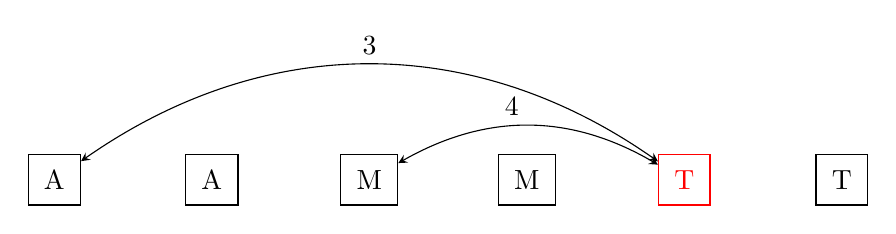
\begin{tikzpicture}[>=stealth]
    \node[rec] (a1) at (0,0) {A};
    \node[rec] (a2) at (2,0) {A};
    \node[rec] (m1) at (4,0) {M};
    \node[rec] (m2) at (6,0) {M};
    \node[red,rec] (t1) at (8,0) {T};
    \node[rec] (t2) at (10,0) {T};
    \draw [<->] (t1) to [bend right=35]node[above]{$3$} (a1);
    \draw [<->] (t1) to [bend right]node[above left]{$4$} (m1);
\end{tikzpicture}
\\We evaluate $TAMUK[4]$: $a=1$ and $m=3$.\\\\
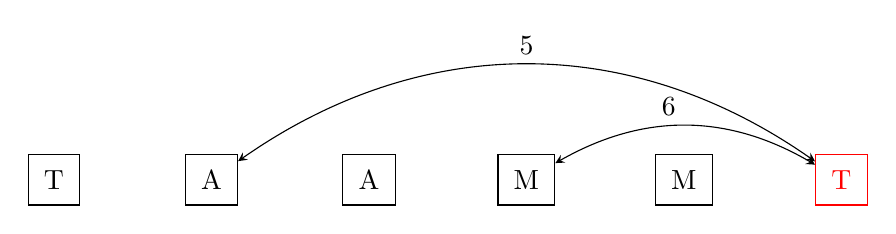
\begin{tikzpicture}[>=stealth]
    \node[rec] (t1) at (0,0) {T};
    \node[rec] (a2) at (2,0) {A};
    \node[rec] (a1) at (4,0) {A};
    \node[rec] (m2) at (6,0) {M};
    \node[rec] (m1) at (8,0) {M};
    \node[red,rec] (t2) at (10,0) {T};
    \draw [<->] (t2) to [bend right=35]node[above]{$5$} (a2);
    \draw [<->] (t2) to [bend right]node[above left]{$6$} (m2);
\end{tikzpicture}
\\We evaluate $TAMUK[5]$: $a=2$ and $m=4$.\\\\
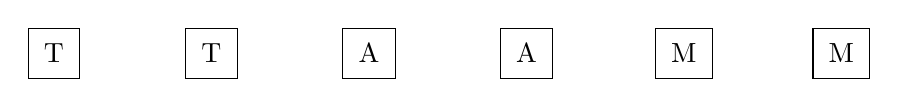
\begin{tikzpicture}[>=stealth]
    \node[rec] (t1) at (0,0) {T};
    \node[rec] (t2) at (2,0) {T};
    \node[rec] (a1) at (4,0) {A};
    \node[rec] (a2) at (6,0) {A};
    \node[rec] (m1) at (8,0) {M};
    \node[rec] (m2) at (10,0) {M};
\end{tikzpicture}
\\The final sorted array. 
Notice that there were 6 swap operations (indicated by the number on the directed edges).
This is not the optimal/minimum number of swaps to sort the array.
Instead, the optimal is shown below:\\
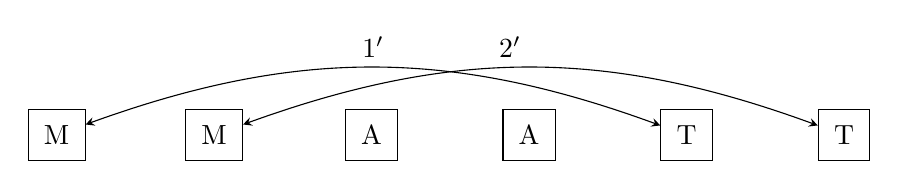
\begin{tikzpicture}[>=stealth]
    \node[rec] (m1) at (0,0) {M};
    \node[rec] (m2) at (2,0) {M};
    \node[rec] (a1) at (4,0) {A};
    \node[rec] (a2) at (6,0) {A};
    \node[rec] (t1) at (8,0) {T};
    \node[rec] (t2) at (10,0) {T};
    \draw [<->] (t1) to [bend right=20]node[above]{$1'$} (m1);
    \draw [<->] (t2) to [bend right=20]node[above left]{$2'$} (m2);
\end{tikzpicture}
\pagebreak
\\This optimal can be achieved by noticing that the swap operations are composible.
Notice that the composition of swap 1, swap 3, and swap 4 is equivalent to swap $1'$, since `A' starts and ends up at $TAMUK[2]$, `M' starts at $TAMUK[0]$ and ends up at $TAMUK[4]$, and `T' starts at $TAMUK[4]$ and ends up at $TAMUK[0]$.
Similarly swap $2'$ is equivalent to the composition of swap 2, 5, and 6. Finding the minimal swap then becomes finding cycles in a graph. Unfortunately, we would then need to store the swaps as edges between vertices (which will be on the same order of magnitude as the array itself), violating constraint 3.

\chapter{Code}

\chapter{Tests}

\chapter{Lessons Learned}

\bibliographystyle{plain}
\bibliography{refs}

% --------------------------------------------------------------
%     You don't have to mess with anything below this line.
% --------------------------------------------------------------
 
\end{document}